\documentclass[conference]{IEEEtran}

\usepackage{indentfirst}
\usepackage{float}
\usepackage{listings}
\usepackage{footnote}
\usepackage[hidelinks]{hyperref}
\usepackage{multirow}
\usepackage{cite}
\usepackage{url}
\usepackage[utf8]{inputenc}
\usepackage[portuguese]{babel}
\usepackage{datetime}
\usepackage[T1]{fontenc}
\usepackage[pdftex]{graphicx}
%\graphicspath{{./Images/}}
\usepackage[table,xcdraw]{xcolor}
\usepackage{adjustbox}
% correct bad hyphenation here
\usepackage{hyphenat}
\hyphenation{mate-mática recu-perar}


\begin{document}

%
%
% ------------------------------------------------------------

\title{How private is my medical information?\\
	\vspace*{10pt} \large Sociologia e Ética da Informática\\
		\normalsize \today{} }
%
\author{Vanessa Silva\\
	{\texttt{(up201305731@fc.up.pt)}}\\
	\multicolumn{1}{p{.7\textwidth}}{\centering\emph{
		\\Departamento de Ciências de Computadores,\\Faculdade de Ciências da Universidade do Porto}}
}

\maketitle

% ------------------------------------------------------------

%----------------------ABSTRACT----------------------%

\begin{abstract}

Perante todo um conjunto de software, bases e bancos de dados, que contém informação médica das pessoas atualmente, tanto para a realização de melhores cuidados de saúde como para investigação, por exemplo, criação de modelos de previsão de doenças, a preocupação de como essa informação é utilizada e se é mantida privada é de extrema relevância e é um dos assuntos mais discutidos atualmente.

\end{abstract}


% ------------------------------------------------------------

\IEEEpeerreviewmaketitle

%----------------------INTRODUÇÃO----------------------%

\section{Introdução}

A gestão da informação médica dos utentes nas instituições de saúde coloca, para além de questões de organização dessa informação, questões éticas, jurídicas, tecnológicas, e principalmente questões de segurança relacionadas com a confidencialidade, integridade e disponibilidade dessa informação.
Isto implica os diferentes profissionais envolvidos, os próprios utentes (a quem os dados dizem respeito), a forma como os registos clínicos são produzidos, armazenados, geridos, tornados acessíveis e partilhados.

Uma crescente preocupação em relação à privacidade de dados pessoais, e em particular os dados médicos, é notória nos dias de hoje. A ideia de privacidade em si não é de todo recente, contudo, com o avanço das novas tecnologia e a sua crescente utilização em áreas como a saúde, para uma melhor gestão, acessibilidade e partilha de informações médicas, cujo intuito é melhorar os cuidados de saúde prestados, essa preocupação tem vindo a acentuar-se dada a quantidade e sensibilidade da informação, que é mantida nos sistemas de informação utilizados nas instituições de saúde.

De forma a promover e a manter os princípios de confidencialidade, integridade e disponibilidade da informação médica, em Portugal, existe um conjunto de organizações, como a CNPD, Ordem dos Médicos, GNS/CNCS e SPMS, que têm como objetivo manter os dados pessoais dos utentes confidenciais, tanto assegurando a obediência das regras de ética e deontologia profissional, como assegurar a utilização segura do ciberespaço e dos meios de partilha de informação.

O avanço das tecnologia trouxe à área da saúde meios que melhoram em muito a qualidade dos cuidados de saúde prestados, dada a rapidez, a acessibilidade e a possibilidade de partilha de informação entre profissionais e instituições de saúde. Contudo, toda a informatização envolvente traz maiores riscos de a informação médica dos utentes ser acedida por pessoas não autorizadas, o que pode levar a crimes (como roubo de identidade), ou discriminação ou exclusão profissional e social. Estes acessos indevidos tem origem em ataques como \textit{phishing} e de \textit{ransomware}, que dizem respeito à cibersegurança, mas também podem ter origem em ataques por parte do profissionais que tem acesso aos dados e os usam de forma indevida.

Em particular, a cibersegurança é um desafio atual para as instituições de saúde uma vez que o número de ameaças bem-sucedidas nestas instituições cresceu significativamente, segundo a SPMS. Sabe-se que, nos Estados Unidos, mais de 110 milhões de registos individuais de saúde foram alvo de ciberataques em instituições hospitalares, um número 3 vezes superior, quando comparado com o total de ameaças ocorridas entre 2009 e 2014.

Atualmente as pesquisas sobre proteção da privacidade dos utentes são centralizadas em torno da proteção do processo clínico eletrónico, ou seja, para que a informação médica do utente seja protegida dos acessos abusivos dos profissionais autorizados, ou dos acessos de pessoas não autorizadas, ou da re-identificação dos dados a partir de dados de saúde publicados para utilizações secundárias.

Perante todo o tratamento, acessibilidade, utilização e partilha a que a informação médica está sujeita, podemos colocar uma série de questões pertinente, como: Quão privada é a minha informação médica? Quem possui e quem tem acesso ao meu processo clínico eletrónico? Como e onde são utilizados os meus dados? Posso colocar restrições sobre quem pode aceder à minha informação médica? Que medidas de segurança são usadas para garantir que a minha informação médica está segura?, neste relatório tentamos responder a estas questões.

O temas abordado neste relatório, vai inteiramente de encontro com os tópicos abordados em três das palestras apresentadas nas aulas, nomeadamente, a palestra sobre Privacidade e Cibersegurança, dada pelo Prof. Luís Filipe Antunes (DCC/FCUP), onde abordou exatamente este assunto da disponibilidade da nossa informação médica aos profissionais de saúde e os riscos consequentes. Também a palestra sobre Privacidade e Proteção de Dados, dada pela Prof. Dra. Filipa Calvão, Presidente da CNPD, o qual referenciamos ao longo do relatório, e a palestra sobre Arquivos de dados de saúde, dada pela Dra. Fernanda Gonçalves, Diretora do Serviço de Arquivo, Segurança e Acesso à Informação do Centro Hospitalar São João (Porto), onde alertou exatamente para alguns dos riscos aqui mencionados, para a necessidade de uma maior consciencialização dos profissionais para este assunto e para o desenvolvimento de sistemas de informação mais seguros, tento desde início a preocupação com "o que o sistema não pode fazer?", também abordou a dualidade apresentada ao longo do trabalho que consiste no peso entre as considerações de saúde pública (graves ameaças, como a gripe da aves) e a manter a privacidade das informações médicas (que podem ser usadas no combate a tais ameaças).

O presente relatório está organizado da seguinte forma, numa primeira parte apresentamos alguns dos termos usados bem como as principais entidades controladoras do sistema de saúde em Portugal (secção \ref{term_ent}), seguindo-se da apresentação da motivação do assunto discutido bem como apresentação dos princípios éticos na área da saúde, definição dos proprietários dos dados relativos às informações médicas, e explicação de como esses dados são tratados e utilizados, na secção \ref{infmed}. Na secção \ref{probseg}, abordamos o tema dos problemas na segurança da informação médica, tanto a nível dos profissionais de saúde e utentes, como das vulnerabilidades dos sistemas de informação. Por último, apresentamos algumas das plataformas e aplicações atualmente usadas na área da saúde (secção \ref{plat_app}), seguindo-se de uma revisão sintética do tema abordado (secção \ref{concl}).


%----------------------TERMINOLOGIA E ENTIDADES DE SAÚDE----------------------%

\section{Terminologia e Entidades de Saúde} \label{term_ent}

Nesta secção vamos apresentar a definição de alguns dos termos usados ao longo do relatório para uma melhor compreensão dos factos, e também a introdução das principais entidades controladoras do sistema de saúde em Portugal.

\subsection{Terminologia}

\begin{itemize}

	\item \textbf{Dados pessoais} - qualquer informação, independentemente da natureza e do respetivo suporte, incluindo som e imagem, relativa a uma pessoa singular identificada ou identificável (titular dos dados); sendo que uma pessoa é considerada identificável pode ser identificada direta ou indiretamente, por referência a um número de identificação ou a um ou mais elementos específicos da sua identidade física, fisiológica, psíquica, económica, cultural ou social \cite{parecerERS2015}, \cite{CNPDinfsaude2014}.
	
	\item \textbf{Informação médica} - informação de saúde destinada a ser utilizada em prestações de cuidados ou tratamentos de saúde \cite{regulamentodeonmedic}.
	
	\item \textbf{Informação de saúde} - qualquer informação direta ou indiretamente ligada à saúde, presente ou futura, de uma pessoa, quer se encontre com vida ou tenha falecido, e a sua história clínica e familiar \cite{consolidacaoinfsaude}.
	
	\item \textbf{Processo clínico} - qualquer registo, informatizado ou não, que contenha informação de saúde sobre utentes ou sobre os seus familiares. Deve conter toda a informação médica disponível que diga respeito ao utente, incluindo a sua situação atual, evolução futura e história clínica e familiar, bem como de informação suficiente sobre a identificação do utente \cite{regulamentodeonmedic}, \cite{parecerERS2015}. 
	
	\item \textbf{Ficha clínica} - é o registo dos dados clínicos do utente e das anotações pessoais do médico. Tem como finalidade a memória futura e a comunicação entre os profissionais que tratem o utente \cite{regulamentodeonmedic}.
	
	\item \textbf{Processo clínico eletrónico} - agrega informação médica dispersa de um utente, pode conter dados relativos à sua história clínica, exames físicos e complementares, diagnósticos, intervenções cirúrgicas, e são introduzidos e visualizados de forma estruturada. Permite a articulação entre vários serviços de saúde, a consulta e o pedido em \textit{real time} de meios complementares de diagnóstico, bem como a partilha da informação entre o utente, os profissionais de saúde e as instituições \cite{CNPDinfsaude2014}.
	
	\item \textbf{Tratamento de dados pessoais} - qualquer operação ou conjunto de operações efetuadas sobre os dados pessoais, com ou sem meios automatizados, tais como recolha, registo, organização, conservação, adaptação ou alteração, recuperação, consulta, utilização, comunicação, bloqueio, eliminação ou destruição \cite{parecerERS2015}.
	
	\item \textbf{Dados anonimizados} - alteração do processo clínico impossibilita a vinculação dos utentes com os seus dados \cite{safran2007toward}.
	
	\item \textbf{Dados de-identificados} - eliminação de todos os identificadores, ou seja, nome do utente, número de utente, número de segurança social, e outros dados que vinculam diretamente um utente com os seus dados \cite{safran2007toward}.
	
	\item \textbf{Dados anonimizados reversíveis} - alteração do processo clínico de forma a que a re-identificação possa ser realizada através do acesso a uma chave protegida que permita vincular os utentes com os seus dados \cite{safran2007toward}.
	
	\item \textbf{Privacidade} - direito fundamental de cada indivíduo de decidir quem deve ter acesso aos seus dados pessoais \cite{segurancaSI}.
	
	\item \textbf{Confidencialidade} - disponibilidade de medidas e mecanismos para manter a privacidade do utente, e proporcionando uma estrutura que permita dar acesso a informação privada, a quem foi dada autorização para tal \cite{segurancaSI}.
	
\end{itemize}


\subsection{Entidades Controladoras do Sistema de Saúde em Portugal}

\begin{itemize}

	\item \textbf{Comissão Nacional de Proteção de Dados (CNPD)}: Entidade administrativa independente, com poderes de autoridade, que funciona junto da Assembleia da República. Tem como função controlar e fiscalizar o cumprimento das disposições legais na matéria de proteção de dados pessoais, em rigoroso respeito pelos direitos do homem e pelas liberdades e garantias consagradas na Constituição e na lei.
	
	\item \textbf{Ordem dos Médicos}: Associação pública que representa os médicos que exercem a profissão em Portugal, distribuídos por especialidades, sub-especialidades e competência, cuja principal missão é promover a defesa da qualidade dos cuidados de saúde prestados à população, bem como o desenvolvimento, a regulamentação e o controlo do exercício da profissão de médico, assegurando a observância das regras de ética e deontologia profissional.
	
	\item \textbf{Gabinete Nacional de Segurança/Centro Nacional de Cibersegurança (GNS/CNCS)}: Tem como principal objetivo contribuir para que o país use o ciberespaço de forma livre, mas, e acima de tudo, de forma confiável e segura, através da promoção de uma contínua melhoria da cibersegurança nacional e da cooperação internacional, bem como da implementação de medidas e instrumentos necessários para antecipar, detetar, reagir e recuperar de situações que, face à ocorrência de incidentes ou ciberataques, ponham em causa o funcionamento das infraestruturas críticas e os interesses nacionais \cite{colabCNCS_SPMS}.
	
	\item \textbf{Serviços Partilhados do Ministério da Saúde (SPMS)}: Tem com principal objetivo a cooperação, a partilha de conhecimento e informação e o desenvolvimento de atividades de prestação de serviços nas áreas dos sistemas e tecnologias de informação e de comunicação, garantindo a operacionalidade e segurança das infraestruturas tecnológicas e dos sistemas de informação do Ministério da Saúde.

\end{itemize}

Dadas as competências particulares e objetivos comuns, no passado dia 21 de fevereiro de 2017, a SPMS assinou com a GNS/CNCS um protocolo de cooperação. Este protocolo visa promover a otimização de procedimentos e uma maior eficiência no sistema, estabelecendo as formas de cooperação entre as partes no desenvolvimento das capacidades nacionais de cibersegurança, troca de conhecimento e aprofundamento das capacidades.


%----------------------INFORMAÇÃO MÉDICA----------------------%

\section{Informação Médica}	\label{infmed}

A recolha da informação médica é feita durante uma consulta médica, essencialmente através da narrativa do utente, de exames complementares e através da consulta ao processo e à ficha clínica anterior do utente, caso existam (figura \ref{fig1}).

A informação que consta num processo clínico corresponde a informação maioritariamente alfanumérica, ou seja, que pode ser representada por carateres ou dígitos. Enquanto que a restante informação, proveniente dos meios complementares de diagnóstico, como sinal ou imagem, normalmente não consta no processo clínico. Por exemplo imagens de ressonâncias magnéticas só são visualizadas quando explicitamente solicitadas, não ficando assim toda a informação clínica de um dado utente disponível como um todo \cite{santos2010comunicaccao}.

Na verdade, muitas das vezes os profissionais de saúde não dispõem de toda a informação sobre os utentes, o que poderá refletir-se na qualidade e nos resultados da sua intervenção. Estas falhas no acesso à informação médica podem conduzir a quebras na continuidade dos serviços prestados, a tratamentos/procedimentos inadequados ou pouco eficazes, com efeitos negativos para o bem-estar do utente \cite{santos2010comunicaccao}. 

\begin{figure}[!t]	
    \centering
    \begin{minipage}{.9\textwidth}
        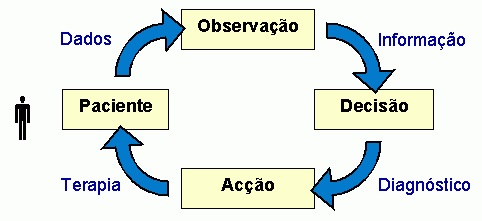
\includegraphics[width=0.53\textwidth]{diagnostico_terapeutica.png}
        \label{fig1}
    \end{minipage}%
    \caption{Ciclo clínico \cite{regclinelect}.}
\end{figure}
 
O processo clínico em papel é uma forma de registo clínico onde os dados são escritos pelo proficional de saude, e toda a informação clínica complementar é anexada a este. Este é um sistema de armazenamento, que serve de base à prestação de cuidados de saúde, e por isso, necessita de integrar informação proveniente de diversas fontes \cite{regclinelect}. Mas com o decorre dos anos o formato em papel começou a desencadear vários inconvenientes devido à diversidade da estruturação da informação, que depende do médico e/ou da instituição, ou a falta dela, devido ao acesso limitado à informação bem como a dificuldades na localização de determinada informação, à ilegibilidade dos registos médicos, e a perdas e duplicação de informação \cite{regclinelect}.

Com o avanço da tecnologia, surgiram os processos clínico eletrónicos que visam não só colmatar as limitações referidas, bem como fornecer uma variedade de ferramentas auxiliares que permitam ajudar na decisão clínica, avaliar a qualidade dos cuidados prestados, ajudar na investigação e na educação médica, realizar a gestão e o planeamento dos recursos de saúde, e possibilitar a troca de informação clínica entre cuidados primários e hospitalares. Mas, em contrapartida, toda esta informatização implica um elevado nível de proteção e segurança, dada a quantidade e sensibilidade da informação clínica e pessoal contida nos processos clínicos eletrónicos.

As preocupações de proteção e segurança derivam do facto de que as diferentes instituições podem partilhar estas informações sensíveis entre si, confiando mutuamente que a informação irá ser mantida confidencial e será apenas usada para o propósito definido, assim como nas trocas de informação entre profissionais da mesma instituição. Contudo, o resultado desta partilha pode não ser o esperado, por isso é de grande preocupação o facto de que estes profissionais podem aceder à informação médica, não só da rede da sua instituição de trabalho como também de outras instituições. Isto torna difícil a gestão e a auditoria de quem tem, ou teve, acesso e a que informação, bem como saber quais os mecanismos de segurança o sistema deve ter.

\begin{table*}[!ht]
\centering
\caption{Técnicas de prevenção e deteção/correção de problemas relacionados com a segurança \cite{segurancaSI}.}
\label{tabl1}
\begin{adjustbox}{max width=\textwidth 	}
\begin{tabular}{ |l|l|l| }

\hline
	\multicolumn{1}{|c|}{\cellcolor[HTML]{EFEFEF}{\color[HTML]{333333}}}	&	\multicolumn{1}{|c|}{\cellcolor[HTML]{EFEFEF}{\color[HTML]{333333} \textbf{Prevenção}}}	&	\multicolumn{1}{|c|}{\cellcolor[HTML]{EFEFEF}{\color[HTML]{333333} \textbf{Deteção/Correção}}}	\\
\hline

\multirow{3}{*}{\textbf{Confidencialidade}}			&	controlar acesso					&	auditoria					\\
													&	autenticação						&	monitorização				\\
													&	encriptação							&								\\
\hline

\multirow{4}{*}{\textbf{Integridade}}				&	assinaturas digitais				&	assinaturas digitais		\\
													&	apoio à introdução de dados			&	auditoria					\\
													&	\textit{standards} e codificações	&	monitorização				\\
													&	métodos de consistências interna	&								\\
\hline

\multirow{4}{*}{\textbf{Disponibilidade}}			&	redundância de equipamento			&	redundância de equipamento	\\
													&	sistemas de recuperação automática	&	auditoria					\\
													&										&	monitorização				\\
													&										&	backups 					\\
\hline

\end{tabular}
\end{adjustbox}
\end{table*}

O problema da segurança nos sistemas de informação é um dos temas mais falados na atualidades, não só relacionados à área da saúde como a todas as outras área. Devemos, ainda, ter especial atenção a problemas relacionado, como a confidencialidade, uma vez que a grande acessibilidade aos dados implica uma grande ameaça para a privacidade dos utentes, devendo-se adotar medidas para prevenir a ocorrência de acessos não autorizados; como a integridade, pois erros nos dados e no software podem acontecer, devendo-se adotar medidas de proteção contra a perda ou corrupção dos dados; e como a disponibilidade, dado que as instituições de saúde ficam cada vez mais dependentes do funcionamento dos sistemas de informação, devendo-se adotar medidas para que o acesso autorizado a informação confidencial esteja disponível sempre que necessário. Ver tabela \ref{tabl1}.

Rapidamente percebemos que para uma melhor proteção da informação deve-se aplicar as medidas de segurança tanto a nível dos equipamentos e do software, como das pessoas e dos procedimentos. Garantir uma segurança perfeita é ainda impossível, no entanto é possível reduzir os riscos ou restringir possíveis danos devido à má utilização e/ou ao uso abusivo dos sistemas de informação.


\subsection{Princípios Éticos} \label{princ_eticos}

Todas as instituições estão sujeitas a princípios éticos, e como tal as ações dos profissionais de saúde estão sujeitas a esses princípios, o qual  destaca o sigilo médico. Adicionalmente, quando estes princípios se aplicam no âmbito da informática, destaca-se desde logo o princípio da privacidade e o princípio da segurança, uma vez que todos os utentes têm o direito à privacidade e ao controlo do tratamento da sua informação médica (como a recolha, o armazenamento, o acesso, o uso e a transmissão), e os dados recolhidos pelos profissionais de saúde devem ser protegidos contra a perda, corrupção, destruição, acesso, uso e alteração indevida ou não autorizada \cite{segurancaSI}.

Perante toda a disponibilidade de informação clínica aos profissionais de saúde, que por um lado é essencial para uma melhor prestação de cuidados, mas que por outro pode ser em demasia e põe em causa questões muito sérias sobre a segurança dos dados. Inclusive, recentemente, o Bastonário da Ordem dos Médicos, Miguel Guimarães, afirmou o seguinte, "Os médicos têm potencialmente acesso a qualquer informação clínica de um utente e nem sei se deviam ter acesso a todas. Mas não são só os médicos que têm acesso, há outros profissionais que também têm", e, em defesa dos médicos, afirma que, "Isto é um problema atual. Mas quem é responsável pela partilha dessa informação de utentes não são os médicos", uma vez que, "Numa questão em que os dados passam a estar disponíveis num local em que potencialmente podem ter vários utilizadores, tenho dúvidas que a responsabilidade dessa partilha deva ser do médico e não do Estado português".

Com vista a melhorar a proteção de dados relacionados à saúde, uma série de leis e regulamentos foram propostos e atualizados nos últimos anos.

Segundo o Regulamento de Deontologia Médica n.º707/2016, de 21 de Julho, "O Código Deontológico da Ordem dos Médicos é um conjunto de normas de comportamento que serve de orientação nos diferentes aspetos das relações humanas que se estabelecem no decurso do exercício profissional da medicina.". Diante destas normas, está bem explícita a obrigatoriedade do segredo médico, quer singular ou coletivamente, em unidades de saúde públicas, sociais, cooperativas ou privadas, no que diz respeito às informações que constem do processo individual do utente. E que é ainda dever das unidades de saúde e dos diretores clínicos impedir o acesso indevido de terceiros aos processos clínicos e aos sistemas informáticos que contenham informação de saúde.
Consoante o artigo 32.º, o dever de segredo médico deixa de ser aplicado apenas e só mediante o consentimento do utente (ou representante legal), se a revelação não prejudicar terceiros com interesse na manutenção do segredo, e não pode ser revelado mais do que o extremamente necessário. O mesmo é válido para as informações que revelem um nascimento ou um óbito, e de doenças de declaração obrigatória (como o caso de epidemias).

Perante o artigo 36.º do regulamento, sobre dados médicos informatizados, todos os ficheiros, bases e bancos de dados com informações clínicas sujeitas a segredo médico, devem ser equipados com sistemas, e utilizados com procedimentos de segurança, que impeçam a consulta, alteração e destruição de dados por pessoas não autorizadas, e que detetem desvios de informação, e caso estas condições não se verifiquem, os equipamentos não devem estar conectados com outros tipos de redes informáticas. E perante o artigo 37.º, é da responsabilidade da gestão dos sistemas garantir a separação entre a informação de médica, genética e a informação pessoal, designadamente através da definição de diversos níveis de acesso. 

Dada a crescente disponibilidade da informação médica e a consequente preocupação com a privacidade dessa informação, em Maio de 2018 entra em vigor o novo Regulamento Geral de Proteção de Dados (RGPD) que vem substituir a atual diretiva e lei de proteção de dados pessoais, o que também inclui a informação relativa a saúde. Perante este novo regulamento, em \cite{rgpd2018} é apresentada uma análise prática sobre o tratamento e acesso a dados de saúde, onde conta que uma instituição de saúde que pretenda recolher e tratar dados pessoais dos seus utentes e dos dados relativos à saúde dos mesmos (dados pessoais relacionados com a saúde física ou mental de uma pessoa singular, incluindo a prestação de serviços de saúde, que revelem informação sobre o estado da sua saúde), deverá obter o consentimento do utente para tais finalidades. Este consentimento consiste "numa manifestação de vontade, livre, específica, informada e explícita, pelo qual o titular dos dados aceita, mediante declaração ou acto positivo inequívoco, que os dados pessoais que lhe dizem respeito sejam objecto de tratamento".


\subsection{Proprietário da Informação Médica}

Perante a lei n.º 12/2005, de 26 de Janeiro, sobre informação genética pessoal e informação de saúde, a informação de saúde, incluindo os dados clínicos registados, resultados de análises e de outros exames, intervenções e diagnósticos, é propriedade do utente, e as instituições de saúde são os depositários dessa informação, sujeitos ao segredo médico. Perante isto, o titular da informação tem o direito de tomar conhecimento dessa informação, presente no seu processo clínico físico e eletrónico, ou de a fazer comunicar a algum terceiro indicado por ele, exceto perante circunstâncias devidamente justificadas.

Uma das restrições excecionais nesta matéria, é a informação constante de anotações pessoais efetuadas pelos profissionais de saúde nos registos e processos clínicos dos utentes.
Pois, tratam-se de anotações pessoais, efetuadas designadamente para memória futura do próprio profissional de saúde, e que não se destinam a classificar ou identificar nenhum dado pessoal do utente.
Assim, tais anotações ou descrições, apesar de poderem constar dos registos e processos clínicos dos utentes, não devem ser considerados dados pessoais dos mesmos.

A CNPD, como autoridade, tem força obrigatória e pode aceder às instalações, aos sistemas informáticos, a ficheiros de dados pessoais e processos clínicos, tendo acesso a qualquer informação médica e pessoal existente, sempre que necessário. O não acatamento das suas decisões configura crime de desobediência qualificada.


\subsection{Utilização e Tratamento de Dados}

Uma das questões mais importantes que todo o utente deve colocar é "Como e onde a minha informação médica é utilizada?".

Primeiramente é importante reconhecermos dois níveis de utilização, utilização primária e utilização secundária de dados. A utilização primária de dados corresponde à utilização da informação de saúde pela instituição que produziu ou adquiriu os dados nela contidos durante o atendimento direto (figura \ref{fig1}), em tempo real, do utente. Enquanto que a utilização secundária de dados corresponde à utilização de técnicas indiretas aplicadas à informação de saúde, incluindo, entre outras, análises, pesquisas, medições de qualidade/segurança, saúde pública, pagamento, certificação ou acreditação de provedores e marketing e outros negócios \cite{safran2007toward}.

É precisamente sobre este segundo nível de utilização que surgem inúmeras questões éticas, técnicas, económicas e processuais que levam à grande questão "\textit{How private is my medical information?}". Uma vez que tanto a indústria como as instituições académicas tem mostrado um grande interesse na utilização da informação médica. 

Entre outros, a utilização para efeitos de investigação, tem ganho amplo interesse dado o surgimento do \textit{Big Data} e \textit{Data Analytics}. Em particular, a construção de modelos de previsão a partir de uma grande conjunto de dados de vários pacientes diferentes, relevantes para uma determinada doença, usando técnicas de \textit{machine learning} pode contribuir substancialmente para a evolução da medicina e para a saúde pública, uma vez que podem ajudar a identificar os fatores de risco genéticos e ambientais e constituir a base para a análise de previsão. No entanto, mesmo utilizando os dados anonimizados, as preocupações com a privacidade devem permanecer \cite{bos2014private}, pois como já mencionado, um processo clínico eletrónico contém para além do conjunto de atributos identificadores (como o nome e o número de utente), atributos "quase"-identificadores (como o género e a morada) e atributos médicos (como doenças), e a partir das técnicas de \textit{data mining} é possível categorizar e pesquisar utentes com base em inúmeros fatores como idade, género ou doença, o que possibilita a re-identificação dos utentes ou subconjuntos de utentes, comprometendo assim a privacidade dos utentes \cite{meingast2006security}.
Dada toda a nova tecnologia e métodos, adotar um nível aceitável de anonimização destes dados (dados de-identificados) tem sido e continua a ser um grande desafio.

Um outro exemplo é o interesse no desenvolvendo de sistemas de sensores para a monitorização remota de utentes, que utiliza tecnologia WBAN (\textit{wireless body area networks}). A ideia é transmitir os dados dos sensores para a estação central de monitorização (o centro de saúde do utente, por exemplo), e incorpora-los no processo clínico eletrónico do utente de forma a melhorar a prestação de cuidados de saúde (ver \cite{meingast2006security} para mais detalhes). Contudo, toda esta tecnologia aumenta o perigo de comprometer a segurança e a privacidade dos utentes, o que leva a uma maior preocupações do que já foi referenciado, ou seja, os direitos de acesso aos dados, como e quando os dados são transferido e armazenados e direitos de análise dos dados.

Isto suscita grande interesse e impacto também económico e, por um lado, temos as empresas privadas que desenvolvem e implantam ferramentas de análise que acumulam dados através dos seus negócios e acordos, e que dependendo desses acordos, podem ou não estar obrigados a manter a confidencialidade dos dados do utentes. Por outro lado, temos verificado um crescente aparecimento de bancos de dados públicos, que apesar de anonimizados, não podemos descartar a possibilidade de re-identificação. Todo este conjunto de bancos de dados trás por uma lado, uma maior exposição da privacidade de todos os utentes o que pode levar a questões sérias como roubo de identidade e discriminação e exclusão, tanto a nível social como profissional, mas por outros grande benefícios para a evolução dos cuidados de saúde, novas descobertas e técnicas de prevenção, e por isso existe uma grande necessidade de encontrar aqui um equilíbrio de forma a minimizar os riscos e aumentar as possibilidades de pesquisa.


%----------------------PROBLEMAS DE SEGURANÇA----------------------%

\section{Problemas de Segurança}	\label{probseg}

Como mencionamos anteriormente, analisar os problemas com a segurança da informação médica é de extrema importância dada a quantidade e qualidade dessa informação que pode ser usada de forma criminosa, como roubo de identidade, e de forma discriminatória, como exclusão perante raças e doenças, tanto a nível social como profissional, e por isso esta informação deve ser confidencial.

Podemos separar o problema com a segurança em dois, o que tem a ver com as vulnerabilidades dos sistemas de informação e o que tem a ver com os problemas com as pessoas, mais precisamente com os profissionais que tem acesso as dados.
E quando ambos os problemas se unificam, ou seja, quando temos sistemas de informação vulneraveis e os proficionais de saúde que os utilizam cometem infrações éticas ao utilizar a infromação médica de forma ilicita para beneficio próprio, o problema é ainda mais complexa e consequentemente mais dificil de resolver. Neste contexto, podemos destacar quatro tipo de ameaças \cite{kayarkar2012classification}:

\begin{itemize}

	\item \textbf{Abuso de privilégios} - acontece quando o utilizador dispõe de mais privilégios do que realmente necessitam.
	
	\item \textbf{Abuso legitimo de privilégios} - acontece quando o utilizador dispõe de privilégios de acesso legítimos, mas intencionalmente explora esses privilégios para aceder a informação de forma maliciosa.
	
	\item \textbf{Promoção de privilégios} - as vulnerabilidades de software e os erros existentes na(s) base(s) de dados e nos sistemas de informação são explorados de maneira a elevar os privilégios do transgressor permitindo-o aceder a informação para o qual não tem acesso.
	
	\item \textbf{Vulnerabilidades do sistema operativo} - o transgressor exploras certas vulnerabilidades do sistema operativo de forma a ganhar acesso não-autorizado à(s) base(s) de dados.

\end{itemize}

No caso dos problemas de segurança relativos às pessoas, a solução vai de encontro com a necessidade de uma maior estimulação, aquando da formação, para o comprimento dos princípios éticos (já mencionados em \ref{princ_eticos}), aplicar, contribuir e rever as normas, políticas e \textit{standards} de segurança de informação, executar auditorias e controlos internos regulares, e realizar ações de sensibilização e de formação para os utilizadores (profissionais de saúde e utentes). Também podem ser tomadas medidas em que o acesso à informação seja ainda mais restrito a estes profissionais, contudo esta medida pode diminuir a eficiência dos cuidados de saúde prestados que tanto se quer aumentar. Por esta razão, a promoção de uma maior disciplina ética é a medida que se deve apostar para combater estes problemas.

Um caso recente que tem a ver exatamente com esta questão de incumprimento da ética, foi o caso da divulgação de informação confidencial sobre o estado de saúde de Marisa Letícia (mulher de Lula da Silva, ex-presidente do Brasil), quando foi internada no Hospital Sírio-Libanês, em São Paulo. Após a sua internação, uma médica do hospital enviou mensagens a um grupo de WhatsApp de antigos colegas de faculdade, confirmando que Marisa Letícia estava nas urgências com diagnóstico de AVC hemorrágico, e rapidamente a mensagem espalhou-se para outros grupos. Um outro médico de fora do Hospital Sírio-Libanês também postou no grupo imagens de uma tomografia atribuída à utente, acompanhada de detalhes que foram confirmados, em seguida, pela médica do Hospital Sírio-Libanês. Os arquivos se espalharam nas redes sociais, inclusive com informações que não constavam no boletim divulgado oficialmente pelo hospital. Perante esta situação a médica foi demitida e alvo de processo de investigação, uma vez que, segundo o presidente do Cremesp (Conselho Regional de Medicina do Estado de São Paulo): "a questão do vazamento de exames, prontuários ou qualquer coisa que revele a doença pela qual a pessoa está passando fere o sigilo médico" quebrando um dos artigo do código de conduta ética.

No caso dos problemas de segurança relacionados com as vulnerabilidades dos sistemas de informação (cibersegurança), existem já uma série de medidas utilizadas para minimizar os problemas, como autenticação, criptografia, controlo e monitorização do acesso e assinaturas digitais. 

Dada a crescente utilização da Web os cuidados que as instituições devem ter a nível de segurança devem ser redobrados. Pois os atacantes possuem grande conhecimento como técnicas de busca e recuperação de informações, que, em junção com a vasta informação que as pessoas colocam \textit{online} (redes social, fóruns, e outras plataformas), torna possível os atacantes descobrirem a identidade e os dados sensíveis de um utente, por exemplo.

Os atacantes possuem técnicas de ataque cada vez mais sofisticadas, levando a um aumento de ameaças em número e em alcance no sector da saúde. Um dos principais ataques utilizados é o \textit{phishing} que se baseia no envio de um email fraudulento com o objetivo de obter dados pessoais ou confidenciais, estes emails são feitos para seres semelhantes às de fontes legítimas, por exemplo, departamento de TIC das instituições hospitalares, instituições financeiras e outras fontes de instituições fidedignas.

Segundo o SPMS, em 2016, variantes destrutivas de \textit{ransomware} como o \textit{Locky} ou o \textit{Samas} infetaram computadores individuais e de empresas, em estabelecimentos de saúde e hospitais em todo o mundo. O \textit{ransomware} é um tipo de software malicioso de encriptação que infecta um computador mostrando alertas que indicam ao utilizador que os seus sistemas foram bloqueados e/ou que os seus arquivos foram encriptados, e restringe o acesso dos utilizadores até que uma quantia de dinheiro seja paga para o desbloquear. 
O \textit{ransomware} é frequentemente transmitido através de emails \textit{phishing} que contêm anexos maliciosos ou através de \textit{drive-by} download, ou seja, quando um utilizador visita um site infetado e, o \textit{malware} é transferido e instalado sem o conhecimento do mesmo \cite{ameacas}. 


%----------------------PLATAFORMAS E APLICAÇÕES----------------------%

\section{Plataformas e Aplicações}	\label{plat_app}

A evolução do exercício da medicina, nomeadamente com a chegada das novas tecnologias obriga os profissionais de saúde a uma constante atualização.

A prescrição eletrónica de medicamentos e os meios complementares de diagnóstico e terapêuticos, representam um passo importante na monitorização e controlo do uso dos recursos tecnológicos na área da saúde. Para estes efeitos e para que haja uma maior interação dos utentes, nos últimos anos têm surgido novas plataformas \textit{online} bem como aplicações para \textit{smartphones}.

Nesta secção vamos apresentar alguma dessas plataformas e aplicações.


\subsection{SONHO}

O SONHO\footnote{\url{http://portalcodgdh.min-saude.pt/index.php/SONHO\#Introdu.C3.A7.C3.A3o}} (Sistema Integrado de Informação Hospitalar) foi desenvolvido com o intuito organizar o sistema de base e dados hospitalares de forma a melhorar a gestão de utentes. É um sistema ADT (\textit{Admission-discharge-transfer}), ou seja, baseia-se na ideia de que a cada utente é atribuído um número único de identificação.

Para além da versão criada para os cuidados hospitalares, SONHO-HOSP V2, que melhora alguns problemas técnicos do SONHO, também foi criada uma versão para os cuidados de saúde primários (SONHO-CSP) que visa cobrir as necessidades administrativas referentes a estes cuidados e que permite, também, um alinhamento entre os cuidados de saúde primários e hospitalares, de extrema importância \cite{sonho}.

O SONHO é constituído por oito módulos (identificação, urgência, internamento, consulta externa, bloco operatório, hospital de dia, arquivo/estatística, e faturação) que melhora a eficiência da gestão dos utentes e dos episódios clínicos. O módulo identificação contém os dados pessoais dos utentes e baseia-se na ideia de "um utente/um número único de identificação" de forma a evitar duplicação de informação; o módulo urgência contêm toda a informação médica sobre a urgência (local e tipo de urgência, tipo de acidente, prioridades, especialidades, etc) e perante está informação liga-se aos módulos de consulta externa, internamento e bloco operatória, é também o único módulo, à exceção do módulo identificação, que permite a existência de dados de identificação de utentes que recorreram ao serviço de urgência e por isso podem não ser ainda utentes do hospital e consequentemente os registos não constam no módulo identificação, estes dados poderão ser posteriormente transcritos para o módulo identificação, caso a urgência gere internamento ou consulta externa \cite{sonho}. O módulo internamento gere alguns procedimentos clínicos e administrativos relacionados com a estadia do utente no hospital, é responsável pela atribuição de cama do utente (consultando o registo de gestão de camas), e caso não existam camas disponíveis deve gerir a respetiva lista de espera, por isso deve conter toda a informação necessária para esta gestão, desde datas (inicio e fim do internamento), especialidades, transferências, diagnósticos, medicamentos, etc, este módulo liga-se ao módulo do bloco operatório e hospital de dia; o módulo hospital de dia gere as agendas das diferentes especialidades e as marcações de sessões, e como tal liga-se ao módulo bloco operatório; o módulo consulta externa gere as tabelas por área de consulta (calcula as demoras médias por médico e especialidade) e gere o calendário e grupos de consulta, estando ligado ao módulo de internamento, bloco operatório e hospital de dia; o módulo bloco operatório contém  informação sobre a gestão de blocos operatórios e salas, quais os motivos de cancelamento de cirurgias,  tipos e grupos de anestesia e respectivos riscos, os tipos de cirurgia, os fármacos por anestesia e faz a gestão dos agendamentos das cirurgias \cite{sonho2013}, \cite{sonho}. O módulo arquivo/estatística é responsável por fornecer o processo do utente, tabelas de grupos, fazer o agrupamento de exames, verificar mapas estatísticos e gerir acessos a mapas por perfil; o modulo faturação permite verificar a faturação de todo o episódio hospitalar e quais as despesas que o cliente terá com o mesmo \cite{sonho}.

Como podemos verificar o SONHO contém toda uma vasta de informação médica e pessoas dos utentes, como informações relativas à própria instituição, e como já mencionado acima isto requer grandes procedimentos e sistemas de segurança. Em particular o SONHO utiliza um sistema de bases de dados que é da Oracle, versão 7.3.4 (atualmente na versão 12) com linguagem PL/SQL (\textit{Oracle’s procedural language extension to SQL}). É manipulada com DBLink (\textit{database link}) que define um caminho "\textit{path}" de uma base de dados da Oracle para outra base de dados, e permite com que sejam feitas "\textit{queries}" em tabelas remotas e executar essas "\textit{queries}" na base de dados. \cite{sonho}. De forma a tornar o sistema seguro, existem políticas de acesso à base de dados e ao sistema, que são geridos localmente sem qualquer gestão central. 

A possibilidade de criação de atalhos para outros sistemas externos através de interfaces WEB podem comprometer a segurança na utilização do sistema e o facto de a tecnologia utilizada no SONHO estar obsoleta \cite{sonho}, implica que existam problemas a níveis aplicacionais tais como na segurança da autenticação, na acessibilidade à informação e monitorização (perfis/utilizador) e na segurança física da informação.


\subsection{SINUS}

O SINUS foi desenvolvido com o objetivo da informatização do perfil administrativo dos Cuidados de Saúde Primários. As sua principais funcionalidades são a gestão de utentes (dados pessoas e de saúde, inscrição na unidade de saúde, atribuição de médico e enfermeiro de família, gestão do processo de família); agendamento de contactos programados e registo de contactos não programados (agendamento de consultas e atos de enfermagem, efetivação, remarcação, gestão de ausências); cobrança de taxas (cálculo de isenções e dispensas de taxas moderadoras e taxas sanitárias, motor de regras para cálculo da cobrança); gestão de utilizadores; gestão de profissionais; gestão de agendas; estatísticas; e listagens \cite{sinus}.

Este sistema é constituído por seis módulos, o que garante a integração de todos dos módulos (módulo integrador), o registo administrativo de contato que contém o registo de todos os contatos do utente com o centro de saúde, o de consulta que contém o registo de informação sobre consultas (a partir do registo administrativo de contato), o módulo de vacinação que contém o plano de vacinas e alertas médicas, o que urgência que regista todas as consultas urgentes e dados decorrentes da urgência (a partir do registo administrativo de contato), e o cartão de identificação do utente do Serviço Nacional de Saúde que é responsável  pela requisição e emissão de cartões e controlo do número nacional único atribuído a cada utente.

Esta tecnologia foi evoluindo ao longo dos anos permitindo aos profissionais de saúde registar dados clínicos, prescrições e outros dados, resultando na implementação de sistemas como o SAM (Sistema de apoio ao Médico), SAPE (Sistema de Apoio à Pratica de Enfermagem), bem como o desenvolvimento de outros módulos de apoio \cite{sinus}.


\subsection{RSE}

O objetivo do Registo de Saúde Eletrónico (RSE) é melhorar a prestação de cuidados de saúde, e para tal reúne dados clínicos de cada utente recolhidos eletronicamente. Este permite o registo e a partilha da informação entre o utente, os profissionais de saúde e as instituições de saúde, tendo em conta os requisitos da CNPD.

O RSE é constituída por quatro portais \cite{rse}:

\begin{itemize}

	\item \textbf{Área do Cidadão} - destinado aos utentes que podem registar na sua área, contactos de emergência, informação sobre hábitos, medicação, alergias e doenças, medições de peso, altura, glicémia, tensão arterial, colesterol, triglicéridos, saturação de oxigénio e de tempo de coagulação do sangue(INR), podem, também, carregar documentos de saúde, partilhar dados de saúde com os profissionais de saúde, marcar consultas via online, realizar pedidos de prescrição de medicação crónica, consultar a sua informações médicas e consultar os dados que constam do Resumo Clínico Único (RCU): alergias, medicação, diagnósticos, cirurgias e vacinação.
	
	\item \textbf{Portal do Profissional} - destinado ao profissionais de saúde (médicos e enfermeiros) e centrado no utente, de forma a que os profissionais tenham acesso à informação médica do utente, incluindo todas a informação que este coloca na sua Área do Cidadão (assim que autorizar). Este portal também permite o acesso do cronograma com todos os contactos efetuados pelo utente, nas diversas instituições do país.
	
	\item \textbf{Portal Institucional} - consiste num \textit{backoffice} para a gestão centralizada do RSE e estatísticas referentes a ele.
	
	\item \textbf{Portal Internacional} - destinado a médicos de outros país da União Europeia, para a consulta do Resumo Clínico Único do utente, mediante a sua prévia autorização.

\end{itemize}


\subsection{RNU}

O Registo Nacional de Utentes (RNU) representa a base de dados de referência para a identificação dos Utentes do Serviço Nacional de Saúde, através do número de Utente. É constituído pela base de dados nacional (repositório central de dados dos utentes do SNS), pela aplicação web (WEBRNU) que gere os dados de identificação dos utentes, e pela plataforma de interoperabilidade que disponibiliza serviços de consulta de dados (Web Services) a um vasto número de entidades e sistemas do SNS, devidamente autorizados para o efeito.


\subsection{My MedicineOne}

O My MedicineOne\footnote{\url{http://www.medicineone.net//}} é mais um software de gestão clínica, idealizado para a prescrição eletrónica e que permite gerir pequenos consultórios de forma autónoma. Em mais detalhe, o software permite a gestão de patologias, o acesso à base de dados nacional do medicamento com alertas de interações medicamentosas e alergias, a prescrição eletrónica de medicamentos, o registo de consultas, a gestão da faturação, gestão de tarefas, gestão de meios complementares de diagnóstico, antecedentes, biometrias, vacinação, referenciação, entre outros. Para tudo isto é necessário acesso a um vasto conteúdo de informação. 

Os módulos clínico são expandidos com diversas fichas de especialidades e com módulos essenciais como a .

Mediante um acordo assinado com a Ordem dos Médicos, em 2015, o MedicineOne (empresa tecnológica que desenvolveu o My MedicineOne) é responsável pelo tratamento de dados, obrigado a respeitar a confidencialidade dos dados que recolhe e a tratar de forma informatizada ou sem meios automáticos todos os dados recolhido, de acordo como as normas estabelecidas pela CNPD, não podendo divulgar, ceder, transmitir ou facultar os dados. É ainda obrigado a permitir ao titular dos dados gratuitamente, o acesso e a correção das informações prestadas assim como a destruição dos dados recolhidos, ter sistemas de segurança que impeçam a consulta, modificação, destruição ou acrescentamento dos dados por pessoa não autorizada a fazê-lo e que permitam detetar desvios de informação, respeitar o sigilo profissional em relação aos dados tratados e não realizar qualquer tipo de interconexão de dados ou tratamento estatístico. Se estes deveres não forem compridos, é da responsabilidade do MedicineOne indemnizar os lesados pelos danos causados, assim como assumir qualquer tipo de responsabilidade do foro contraordenacional, civil e criminal.


\subsection{iMED}

O iMED\footnote{\url{https://www.imed.pt/imed/}} é uma plataforma de gestão clínica \textit{online} concebida para reunir, num único software, todas as ferramentas essenciais para um simples, completo e eficiente funcionamento de um consultório ou clínica. Este funciona em tecnologia totalmente web, alojada na \textit{Cloud}, sendo apenas necessária uma ligação à Internet para aceder ao sistema.

Esta plataforma dispõe de uma aplicação móvel e de apoio presencial e/ou telefónico gratuito, e, dado o seu objetivo, possui ligação instantânea ao RNU, assim como diferentes níveis de acesso para o staff médico e administrativo, com o intuito de melhorar a segurança e consequente privacidade dos utentes.

Mediante o acordo assinado com a Ordem do Médicos, em 2015, o iMED tem exatamente as mesma obrigações, sobre o tratamento de dados dos utentes, que os mencionado a cima para o MedicineOne.


\subsection{MySNS Carteira}

A App MySNS Carteira\footnote{\url{https://www.sns.gov.pt/apps/mysns-carteira-eletronica-da-saude/}} é uma aplicação oficial do Serviço Nacional de Saúde e tem o objetivo de ser a "A Carteira eletrónica da Saúde". Esta permite que os utentes acedam a um conjunto de funcionalidades, através do \textit{smartphone}, como receber notificações, consultar vacinas, alergias, testamento vital, guias de tratamento, entre outras. Para além destas consultas, permite efetuar uma melhor monitorização dos dados de saúde e guardar informações no \textit{smartphone}.

Através desta aplicação o utente pode gerir a autorização da partilha de informação com profissionais de saúde, em tempo real, através da Área do Cidadão (por exemplo, autorizar antes de uma consulta e desautorizar no final da mesma), cumprindo os requisitos da CNPD.
Também tem a capacidade de realizar sugestões inteligentes, baseadas no contexto clínico do cidadão, localização, hora do dia ou estado do tempo, através de notificações, melhorando assim em muito os cuidados prestados aos utentes.



%----------------------CONCLUSÃO----------------------%

\section{Conclusões}	\label{concl}

Atravessamos um período de transformação digital onde temos cada vez mais informação de carácter pessoal a circular em formato eletrónico, cada vez mais dispositivos pessoais ligados à Internet a qualquer hora e em qualquer lugar, e cada vez mais dependência da Internet, isto acontece tanto a nível pessoal como a nível institucional, e a área da saúde não é exceção.	

O registo eletrónico dos dados clínicos dos utentes e a sua partilha entre todos os profissionais envolvidos é fundamental para melhorar os serviços de cuidados de saúde. Contudo, a privacidade desta informação, como podemos analisar, não é garantida e existe ainda muito trabalho a ser feito a este nível, tanto sobre a consciencialização e disciplina dos profissionais envolventes como de mecanismos de segurança informática mais sofisticados e eficientes.

Todo este trabalho é inevitável dada a importância de conseguir um bom compromisso entre os dois principais objetivos que, como analisado, entram em conflito: melhorar os cuidados de saúde prestados e garantir a privacidade dos seus dados. E de forma a comprovar essa necessidade e o atual interesse neste assunto, várias ideias e iniciativas têm sido propostas recentemente. O novo Regulamento Geral de Proteção de Dados, já mencionado é um deles, mas também a criação do Centro de Desenvolvimento e Capacitação em Cibersegurança na Saúde\footnote{\url{http://www.atlasdasaude.pt/publico/content/coimbra-recebe-centro-de-formacao-em-ciberseguranca-na-saude}} e a criação do NanoSTIMA (\textit{Macro-to-Nano Human Sensing: Towards Integrated Multimodal Health Monitoring and Analytics})\footnote{\url{http://www.90segundosdeciencia.pt/episodes/ep-274-pedro-rodrigues/}}, são exemplos de grandes projetos recentes que mostram o grande interesse no assunto que foi analisado neste relatório.


\bibliography{referencias_PMI}{}
\bibliographystyle{IEEEtran}

\end{document}
